% -*- root: ../../main.tex -*-
\section{Interazioni}
\label{sec:interactions_design}

\subsubsection{Interazione tra Engine, ECS e controller}

%- Il GameEngine rappresenta il gestore di gioco contiene:coordinator che rappresenta l'entry point per le entità fondamentali di ECS - Il motore di gioco è in un modulo a parte (game loop- flusso di controllo a parte) - scopo: aggiornamento dei sistemi mantenendo costanti e modificabili gli fps - si interfaccia con il mediator - GL ha una visione limitata del gameEngine, attraverso updatable engine 




Come spiegato in \ref{sec:ecs_design}, i vari gestori di componenti che formano l'ECS sono coordinati tra di loro tramite un \texttt{Coordinator}. Esso fa da punto di contatto con l'\texttt{Engine}, che rappresenta il gestore della partita e contiene:
\begin{itemize}
    \item \textbf{Coordinator:} è l'entry point per interagire con le entità fondamentali di ECS, esponendo il metodo \texttt{updateAllSystems};
    \item \textbf{GameLoop:} modellato come un flusso di controllo separato, è l'effettivo motore del gioco. Ha una visione limitata dell'engine, \texttt{UpdateableEngine}, su cui richiama ciclicamente update, causando l'aggiornamento dei sistemi, mantenendo costanti e modificabili gli fps mostrati all'utente;
    \item \textbf{Mediator:} consente al gioco di far comunicare \textbf{Engine} e il GameScreen in modalità single-player, mentre al join di una partita multiplayer come client l'engine verrà staccato da parte del controller e il mediator comunicherà con l'attore client. Invece, durante l'hosting di una partita multiplayer il server si affianca al \texttt{GameScreen} e tramite il \texttt{Mediator} riceve gli eventi dall'\texttt{Engine} e li comunica ai client partecipanti alla partita.
\end{itemize}

\begin{figure}[H]
	\centering
	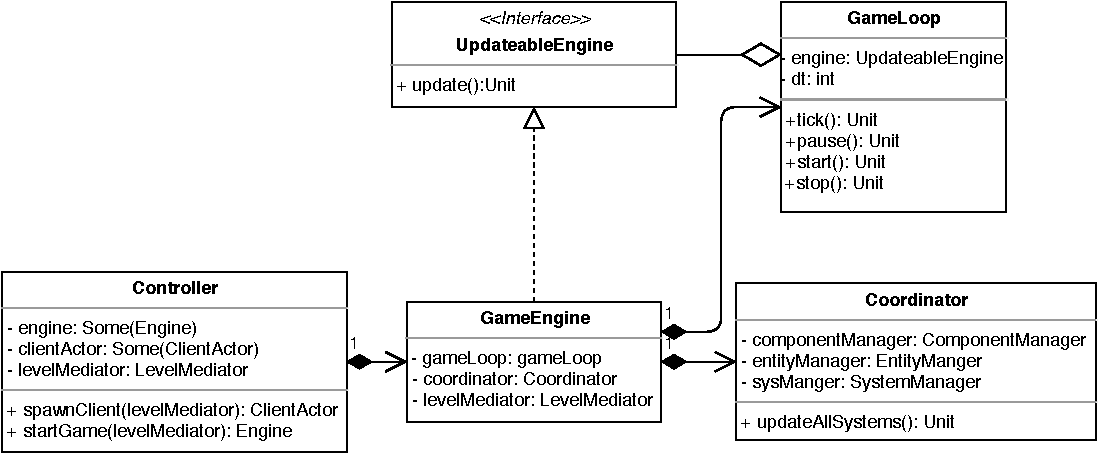
\includegraphics[width=\columnwidth]{drawio/ECS-engine-controller/ecs-engine-controller.pdf}
	\caption{Diagramma raffigurante ecs, engine e controller e le loro interazioni.}
	\label{fig:ecs-engine-controller}
\end{figure}



\subsubsection{Interazione tra Controller e View}
Per rendere possibile l'aggiornamento della View da parte del controller è stato utilizzato il pattern observer, fornendo al controller un oggetto che implementa il trait \textbf{ObserverUI}. Esso fornisce al controller la possibilità di per poter comandare la view in tre scenari principali:


\begin{itemize}
    \item \textbf{Aggiornamento impostazioni globali:} quando l'utente cambia impostazioni globali, o quando vengono caricati i valori di default permette alla view di essere aggiornata con i valori correnti;
    
    \item \textbf{Aggiornamento impostazioni multiplayer:} è necessario poter mos-trare ogni nuovo status della lobby, sia quando si unisce un nuovo giocatore alla partita sia al cambiamento dello stato di "ready" di un giocatore. Inoltre aggiorna i client sui cambiamenti delle impostazioni globali della partita effettuati lato server, che vengono anche essi mostrati nella schermata della lobby;
    
    \item \textbf{Notifica di avvio partita multiplayer:} quando l'host della partita decide di avviarla è necessario far cambiare schermata ai client e fargli caricare il loro GameScreen;
    
\end{itemize}

Invece, per garantire la possibilità alla view di comunicare al controller le operazioni necessarie al setup delle differenti modalità di gioco gli viene fornito il trait \textbf{ObservableUI} che permette le seguenti operazioni:
\begin{itemize}
    \item \textbf{attachUI, detachUI:} quando viene fatto eseguire il gioco in modalità server "headless" è necessario staccare la view, mentre al setup è necessario attaccarla al resto del sistema;
    \item \textbf{loadAllLevels, loadStats, saveStats:} durante la modifica e il caricamento delle impostazioni e delle statistiche, consentono alla view di caricarle da file e modificarle;
    \item \textbf{becomeHost, startMultiplayer, shutDownMultiplayer:}
    
    
    permettono lo switch tra le varie modalità di gioco, e causano il setup o la distruzione dei vari componenti associati;
    \item \textbf{tryJoinLobby, kickSomeone, leaveLobby:} permettono l'interazione con la lobby in modalità multiplayer;
    \item \textbf{start, startMultiplayer:} in modalità singleplayer e in modalità multiplayer quando si è host, notificano al controller l'intenzione dell'utente di iniziare una partita;
\end{itemize}




\begin{figure}[H]
	\centering
	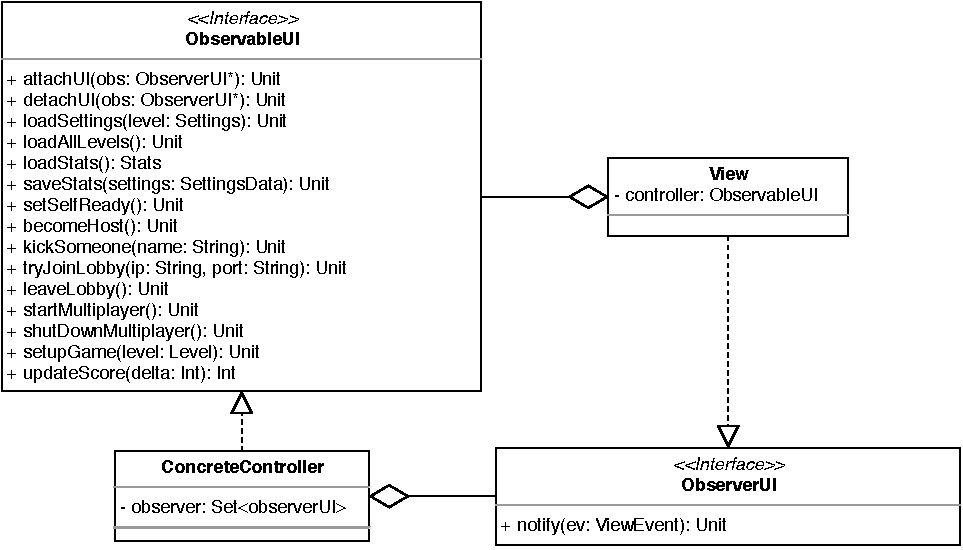
\includegraphics[width=\columnwidth]{drawio/view-controller-observer/view-controller-observer.pdf}
	\caption{Diagramma raffigurante view, controller e observer e le loro interazioni.}
	\label{fig:view-controller-observer}
\end{figure}